\renewcommand{\one}{fake_010}
\renewcommand{\two}{fake_006}
\renewcommand{\thr}{fake_015}
\newcommand{\IDone}{27}
\newcommand{\IDtwo}{27}
\newcommand{\IDthr}{27}

\setlength{\resLen}{.545in}
\begin{figure*}[t]
	\addtolength{\tabcolsep}{-4pt}
	\begin{tabular}{ccccc@{\hspace{4\tabcolsep}}cccc@{\hspace{4\tabcolsep}}cccc}
		\raisebox{.31in}{\rotatebox[origin=c]{90}{\footnotesize{GT Novel}}} &
		\raisebox{0.1in}{\includegraphics[height=\resLen]{results/multi/\one/ref/\IDone.jpg}} &
		\multicolumn{3}{l}{\includegraphics[height=1.7\resLen]{results/multi/\one/err.pdf}} &
		\raisebox{0.1in}{\includegraphics[height=\resLen]{results/multi/\two/ref/\IDtwo.jpg}} &
		\multicolumn{3}{l}{\includegraphics[height=1.7\resLen]{results/multi/\two/err.pdf}} &
		\raisebox{0.1in}{\includegraphics[height=\resLen]{results/multi/\thr/ref/\IDthr.jpg}} &
		\multicolumn{3}{l}{\includegraphics[height=1.7\resLen]{results/multi/\thr/err.pdf}}
		\\
		& \textbf{\small N=1} & \textbf{\small 5} & \textbf{\small 9} & \textbf{\small 25}
		& \textbf{\small N=1} & \textbf{\small 5} & \textbf{\small 9} & \textbf{\small 25}
		& \textbf{\small N=1} & \textbf{\small 5} & \textbf{\small 9} & \textbf{\small 25}
		\\
		\raisebox{.25in}{\rotatebox[origin=c]{90}{\footnotesize{Ours}}} &
		\includegraphics[height=\resLen]{results/multi/\one/ours+_1/\IDone.jpg} &
		\includegraphics[height=\resLen]{results/multi/\one/ours+_5/\IDone.jpg} &
		\includegraphics[height=\resLen]{results/multi/\one/ours+_9/\IDone.jpg} &
		\includegraphics[height=\resLen]{results/multi/\one/ours+_25/\IDone.jpg} &
		\includegraphics[height=\resLen]{results/multi/\two/ours+_1/\IDtwo.jpg} &
		\includegraphics[height=\resLen]{results/multi/\two/ours+_5/\IDtwo.jpg} &
		\includegraphics[height=\resLen]{results/multi/\two/ours+_9/\IDtwo.jpg} &
		\includegraphics[height=\resLen]{results/multi/\two/ours+_25/\IDtwo.jpg} &
		\includegraphics[height=\resLen]{results/multi/\thr/ours+_1/\IDthr.jpg} &
		\includegraphics[height=\resLen]{results/multi/\thr/ours+_5/\IDthr.jpg} &
		\includegraphics[height=\resLen]{results/multi/\thr/ours+_9/\IDthr.jpg} &
		\includegraphics[height=\resLen]{results/multi/\thr/ours+_25/\IDthr.jpg}
		\\
		\raisebox{.25in}{\rotatebox[origin=c]{90}{\footnotesize{Ours+}}} &
		\includegraphics[height=\resLen]{results/multi/\one/ours+_egsr_1/\IDone.jpg} &
		\includegraphics[height=\resLen]{results/multi/\one/ours+_egsr_5/\IDone.jpg} &
		\includegraphics[height=\resLen]{results/multi/\one/ours+_egsr_9/\IDone.jpg} &
		\includegraphics[height=\resLen]{results/multi/\one/ours+_egsr_25/\IDone.jpg} &
		\includegraphics[height=\resLen]{results/multi/\two/ours+_egsr_1/\IDtwo.jpg} &
		\includegraphics[height=\resLen]{results/multi/\two/ours+_egsr_5/\IDtwo.jpg} &
		\includegraphics[height=\resLen]{results/multi/\two/ours+_egsr_9/\IDtwo.jpg} &
		\includegraphics[height=\resLen]{results/multi/\two/ours+_egsr_25/\IDtwo.jpg} &
		\includegraphics[height=\resLen]{results/multi/\thr/ours+_egsr_1/\IDthr.jpg} &
		\includegraphics[height=\resLen]{results/multi/\thr/ours+_egsr_5/\IDthr.jpg} &
		\includegraphics[height=\resLen]{results/multi/\thr/ours+_egsr_9/\IDthr.jpg} &
		\includegraphics[height=\resLen]{results/multi/\thr/ours+_egsr_25/\IDthr.jpg}
		\\
		\raisebox{.25in}{\rotatebox[origin=c]{90}{\footnotesize{[Gao19]+}}} &
		\includegraphics[height=\resLen]{results/multi/\one/msra+_1/\IDone.jpg} &
		\includegraphics[height=\resLen]{results/multi/\one/msra+_5/\IDone.jpg} &
		\includegraphics[height=\resLen]{results/multi/\one/msra+_9/\IDone.jpg} &
		\includegraphics[height=\resLen]{results/multi/\one/msra+_25/\IDone.jpg} &
		\includegraphics[height=\resLen]{results/multi/\two/msra+_1/\IDtwo.jpg} &
		\includegraphics[height=\resLen]{results/multi/\two/msra+_5/\IDtwo.jpg} &
		\includegraphics[height=\resLen]{results/multi/\two/msra+_9/\IDtwo.jpg} &
		\includegraphics[height=\resLen]{results/multi/\two/msra+_25/\IDtwo.jpg} &
		\includegraphics[height=\resLen]{results/multi/\thr/msra+_1/\IDthr.jpg} &
		\includegraphics[height=\resLen]{results/multi/\thr/msra+_5/\IDthr.jpg} &
		\includegraphics[height=\resLen]{results/multi/\thr/msra+_9/\IDthr.jpg} &
		\includegraphics[height=\resLen]{results/multi/\thr/msra+_25/\IDthr.jpg}
	\end{tabular}
	\caption{\label{fig:results_multi_inputs2}
		\revision{\textbf{Performance using different numbers of input images (synthetic data).} 
			The quality of recovered SVBRDF maps, as demonstrated by the plots, generally improves with more input images for both our and Gao's~\shortcite{Gao2019} methods.
			Our method with constant (Ours) and neural (Ours+) initializations are comparable or better than Gao's  ([Gao19]+) with neural initialization~\cite{Deschaintre2019} .
			For a highly specular material shown on the right, although the LPIPS metric computed using renderings under 5 novel views of our results is similar to that of Gao's, ours better preserve the specular highlight.
			For each material, all the renderings including the references (GT Novel) are generated using one of the 5 novel views.
		}
	}
\end{figure*}